\chapter{p-ब्लॉक II: ऑक्सीजन, हैलोजन और उत्कृष्ट गैसें}\label{ch:b1:p-block-16-18}

सल्फ़्यूरिक अम्ल किसी भी अन्य रसायन से अधिक टन-मात्रा में बनाया जाता है: वह
उर्वरकों के लिए फ़ॉस्फ़ेट चट्टान को घोलता है, कॉपर और यूरेनियम अयस्कों का निक्षालन करता है,
तेल का परिष्करण करता है और कार बैटरियाँ भरता है, और एक शताब्दी तक
सल्फ़्यूरिक अम्ल का उत्पादन किसी देश के उद्योग का एक मोटा माप था। अब उसका अधिकांश
सल्फ़र प्राकृतिक गैस और तेल की सफ़ाई से आता है; कुछ अब भी
ज्वालामुखी क्रेटरों से हाथ से ढोकर निकाला जाता है। सल्फ़र \omterm{def:b1:periodicity:table}{समूह} 16 में
ऑक्सीजन के नीचे है; \omterm{def:b1:periodicity:table}{समूह} 17 के \omterm{def:b1:p-block-16-18:halogen}{हैलोजन} और \omterm{def:b1:periodicity:table}{समूह} 18 की उत्कृष्ट गैसें
\omterm{def:b1:periodicity:table}{p-ब्लॉक} को पूरा करती हैं। यह अध्याय ऑक्सीजन और सल्फ़र का तत्त्व से
अम्ल तक अनुसरण करता है, \omterm{def:b1:p-block-16-18:halogen}{हैलोजनों} को उनके \omterm{def:b1:nernst:electrode-potential}{मानक विभवों} द्वारा \omterm{def:b1:nernst:couple}{ऑक्सीकारकों} के रूप में क्रम देता है,
और उन यौगिकों पर समाप्त होता है जो तथाकथित अक्रिय उत्कृष्ट गैसें सचमुच बनाती हैं।

\begin{recall}
\omterm{def:b1:lewis-resonance-vsepr:lewis}{लुइस संरचनाएँ}, विस्तारित अष्टक और VSEPR आकृतियाँ (\cref{ch:b1:lewis-resonance-vsepr});
\omterm{def:b1:nernst:electrode-potential}{मानक विभव} (\cref{ch:b1:nernst}); क्लोरीन का \omterm{def:b1:e-ph-diagrams:disproportionation}{असमानुपातन}
और क्लोरीन का \omterm{def:b1:e-ph-diagrams:e-ph-diagram}{विभव--pH आरेख}
(\cref{ch:b1:e-ph-diagrams}); उत्प्रेरण (\cref{ch:b1:elementary-steps})।
विद्यालय के खंड (कक्षा 10) ने \omterm{def:b1:p-block-16-18:halogen}{हैलोजनों} और उत्कृष्ट गैसों को
कुलों के रूप में समूहित किया था।
\end{recall}

\begin{omfigure}
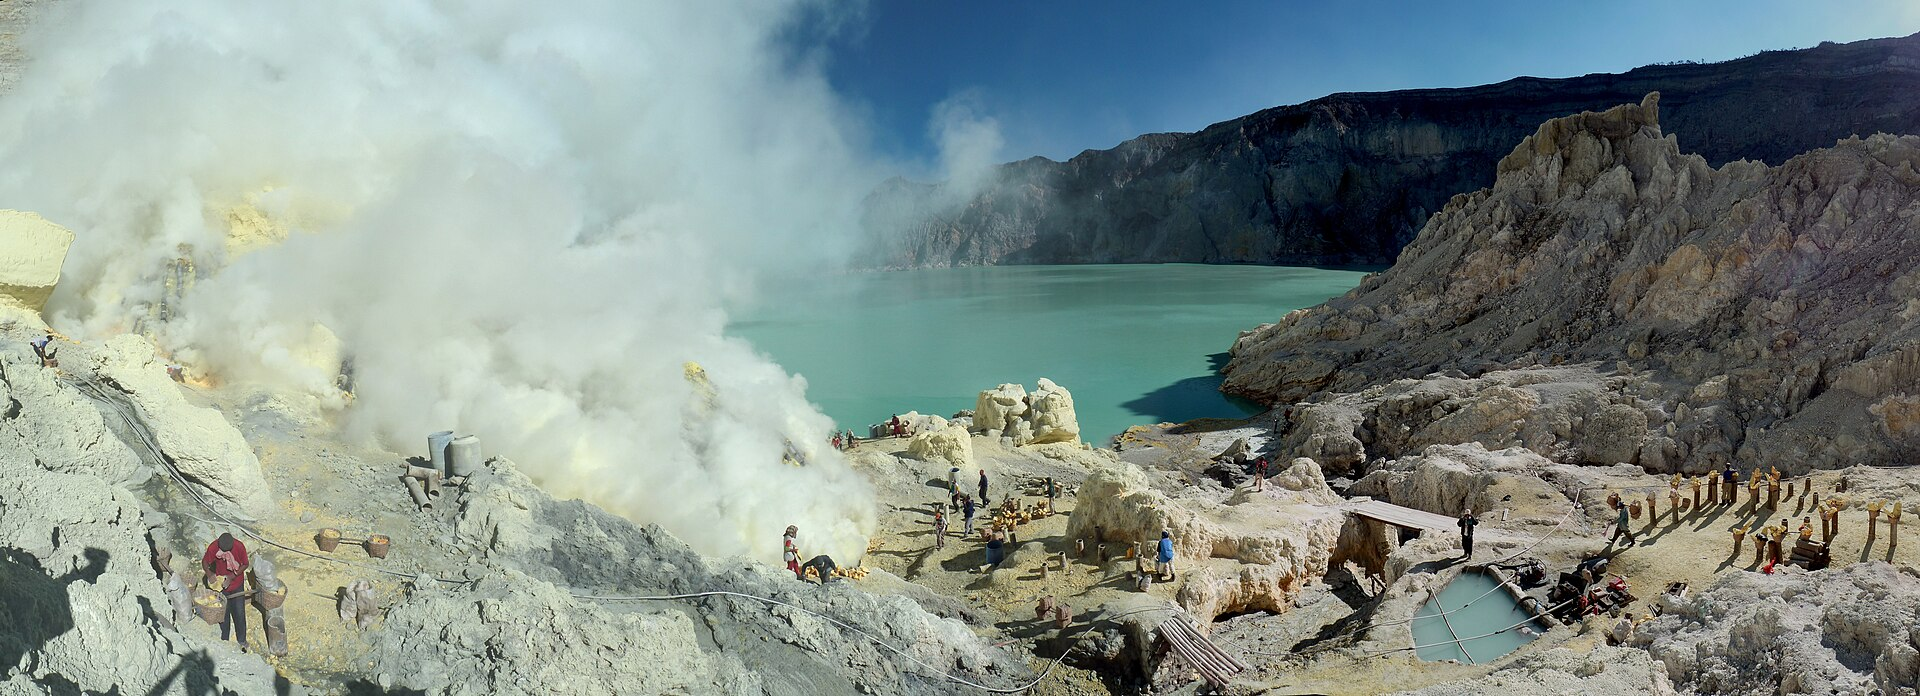
\includegraphics[width=0.78\linewidth]{images/book2/kawah-ijen.jpg}

{\small इंडोनेशिया के कावाह इजेन ज्वालामुखी के क्रेटर में सल्फ़र खनन:
ज्वालामुखी गैसें पाइपों के चारों ओर पीला सल्फ़र संघनित करती हैं, और खनिक उसे
टोकरियों में ढोकर बाहर लाते हैं (छायाचित्र: सेमूर, CC BY-SA 4.0, विकिमीडिया कॉमन्स)।}
\end{omfigure}

\section{ऑक्सीजन, ओज़ोन और पेरॉक्साइड}

\begin{definition}[कैल्कोजन]\label{def:b1:p-block-16-18:chalcogen}
\emph{कैल्कोजन}\index{कैल्कोजन} \omterm{def:b1:periodicity:table}{समूह} 16 के तत्त्व हैं
(O, S, Se, Te, Po), जिनमें छह \omterm{def:b1:quantum-numbers:configuration}{संयोजकता इलेक्ट्रॉन} \textit{ns}$^2$\textit{np}$^4$ होते हैं।
वे $-$II (ऑक्साइड, सल्फ़ाइड) से $+$VI (सल्फ़ेट) तक की \omterm{def:b1:nernst:oxidation-number}{ऑक्सीकरण संख्याओं} वाले
यौगिक बनाते हैं, उच्चतर संख्याएँ केवल सल्फ़र और उसके नीचे के तत्त्वों के लिए।
\end{definition}

ऑक्सीजन डाइऑक्सीजन \ce{O2} के रूप में और ओज़ोन \ce{O3} के रूप में अस्तित्व में है, जो
दो \omterm{def:b1:lewis-resonance-vsepr:resonance}{अनुनादी संरचनाओं} वाला एक कोणीय अणु है (\cref{ch:b1:lewis-resonance-vsepr})। ओज़ोन
डाइऑक्सीजन से अधिक प्रबल \omterm{def:b1:nernst:couple}{ऑक्सीकारक} है: $E^\circ(\ce{O3}/\ce{O2}) = 2.07$~V,
जबकि \ce{O2}/\ce{H2O} के लिए 1.23~V। ऊपरी वायुमंडल में वह
पराबैंगनी प्रकाश अवशोषित करती है; धरातल के पास वह एक प्रदूषक है। हाइड्रोजन पेरॉक्साइड,
जिसमें एक \ce{O-O} आबंध है और ऑक्सीजन $-$I पर है, \omterm{def:b1:nernst:couple}{ऑक्सीकारक} और \omterm{def:b1:nernst:couple}{अपचायक} दोनों है
और धीरे-धीरे असमानुपातित होता है (\cref{exo:b1:nernst:12})।
% ledger: dfg:O3_g (E0 computed in figdata/bachelor-1/standard-potentials.py)

\begin{example}[ऑक्सीजन की ऑक्सीकरण संख्याएँ]
ऑक्सीजन, जो \omterm{def:b1:periodicity:electronegativity}{विद्युत-ऋणात्मकता} में केवल फ़्लुओरीन से पीछे है, अपने लगभग सभी यौगिकों में
$-$II पर है: जल, ऑक्साइड, हाइड्रॉक्साइड, सल्फ़ेट। अपवाद
इस नियम से निकलते हैं कि साझा इलेक्ट्रॉन अधिक विद्युत-ऋणात्मक भागीदार को जाते हैं
और सर्वसम परमाणुओं के बीच बराबर बँटते हैं।
हाइड्रोजन पेरॉक्साइड \ce{H2O2}, H--O--O--H, में हर ऑक्सीजन अपने \ce{O-H} आबंध के
इलेक्ट्रॉन लेता है पर \ce{O-O} युग्म बाँटता है: $-$I। पोटैशियम
सुपरऑक्साइड \ce{KO2} में आयन \ce{O2-} दो परमाणुओं के लिए एक आवेश वहन करता है:
औसतन $-\frac12$। ऑक्सीजन डाइफ़्लुओराइड \ce{OF2} में फ़्लुओरीन दोनों
आबंध जीत लेता है और ऑक्सीजन $+$II पर होता है। \ce{O2} और \ce{O3} में वह 0 पर है। केवल
$-$II अवस्था जल के प्रति स्थायी है; पेरॉक्साइड और सुपरऑक्साइड
\omterm{def:b1:nernst:couple}{ऑक्सीकारक} हैं, और \ce{OF2} एक फ़्लुओरीनकारी अभिकर्मक।
\end{example}

\section{सल्फ़र और सल्फ़्यूरिक अम्ल}

ऑक्सीजन के विपरीत, सल्फ़र एकल \ce{S-S} आबंधों की वलय और शृंखलाएँ बनाता है:
साधारण सल्फ़र \ce{S8} वलयों से बना है। वह जलकर सल्फ़र डाइऑक्साइड देता है, एक
कोणीय अणु (O--S--O कोण \ang{119.5}), जिसे आगे
सल्फ़र ट्राइऑक्साइड तक ऑक्सीकृत किया जा सकता है, जो त्रिकोणीय समतलीय है। दोनों \omterm{def:b1:s-block:oxide-character}{अम्लीय ऑक्साइड} हैं: \ce{SO2}
सल्फ़्यूरस अम्ल देता है ($\mathrm{p}K_a$ 1.77 और 7.22), \ce{SO3} सल्फ़्यूरिक
अम्ल।
% ledger: geo:SO2.aOSO, dfg:SO2_g, dfg:SO3_g

\begin{proposition}[संपर्क प्रक्रम के चरण]\label{prop:b1:p-block-16-18:contact-steps}
सल्फ़्यूरिक अम्ल सल्फ़र से चार चरणों में बनाया जाता है:
(1) \ce{S + O2 -> SO2}; (2) \ce{2SO2 + O2 <=> 2SO3}, वैनेडियम(V)
ऑक्साइड \omterm{def:b1:elementary-steps:catalyst}{उत्प्रेरक} पर; (3) \ce{SO3 + H2SO4 -> H2S2O7} (ओलियम), ट्राइऑक्साइड को
सांद्र अम्ल में अवशोषित करके; (4) \ce{H2S2O7 + H2O -> 2H2SO4}। कुल मिलाकर,
\ce{2S + 3O2 + 2H2O -> 2H2SO4}।
\end{proposition}

\begin{proof}
हर चरण संतुलित है; $2\times(1)$, (2), $2\times(3)$ और
$2\times(4)$ जोड़ने पर, \ce{SO2}, \ce{SO3} और \ce{H2S2O7} निरस्त हो जाते हैं, और चरण 3 में खपे दोनों
\ce{H2SO4} चरण 4 में पुनर्जनित होते हैं, जिससे
\ce{2S + 3O2 + 2H2O -> 2H2SO4} बचता है। चरण 2 कमरे के ताप पर ऊष्मागतिक रूप से अत्यंत
अनुकूल है (\qty{25}{\celsius} पर $K = 10^{24.8}$, निर्माण
गिब्ज़ ऊर्जाओं से) पर अत्यधिक धीमा: \omterm{def:b1:elementary-steps:catalyst}{उत्प्रेरक}, जो केवल गरम होने पर
सक्रिय है, ही उसे चलाता है, और दर तथा रूपांतरण के बीच के समझौते का
अध्ययन द्वितीय वर्ष के खंड में है। \ce{SO3} सीधे जल में
अवशोषित नहीं किया जाता, क्योंकि जलवाष्प के साथ उसकी अभिक्रिया अम्ल की बूँदों की
ऐसी महीन धुंध बनाती है जो अवशोषकों से निकल जाती है।
\end{proof}
% ledger: dfg:SO2_g, dfg:SO3_g

\begin{omfigure}
\begin{tikzpicture}[font=\small, >={Stealth}, box/.style={draw, rounded corners, fill=omDef!8, align=center, minimum height=1.0cm}]
  \node[box] (b) at (0,0) {सल्फ़र दाहक\\\ce{S + O2 -> SO2}};
  \node[box] (c) at (4.4,0) {परिवर्तक, \ce{V2O5}\\उत्प्रेरक संस्तर};
  \node[box] (a) at (8.8,0) {अवशोषण मीनार\\\ce{SO3}, \ce{H2SO4} में};
  \node[box] (d) at (8.8,-2.2) {तनुकरण\\\ce{H2S2O7 + H2O}};
  \draw[<-, thick] (b.west) -- ++(-0.8,0) node[left] {वायु, S};
  \draw[->, thick] (b) -- node[above] {\ce{SO2}} (c);
  \draw[->, thick] (c) -- node[above] {\ce{SO3}} (a);
  \draw[->, thick] (a) -- node[right] {ओलियम} (d);
  \draw[->, thick] (d.west) -- ++(-1.2,0) node[left] {\ce{H2SO4}};
  \draw[->, thick] (d.east) -- ++(0.6,0) |- node[pos=0.25, right] {भाग वापस} (a.east);
\end{tikzpicture}

{\small संपर्क प्रक्रम: सल्फ़र का दहन, \ce{SO2} का उत्प्रेरकी
ऑक्सीकरण, सांद्र सल्फ़्यूरिक अम्ल में \ce{SO3} का अवशोषण, और
ओलियम का तनुकरण। अम्ल का एक भाग अवशोषक में लौटा दिया जाता है।}
\end{omfigure}

\begin{proposition}[सल्फ़्यूरिक अम्ल की प्रबलता]\label{prop:b1:p-block-16-18:sulfuric-strength}
जल में सल्फ़्यूरिक अम्ल की पहली अम्लता प्रबल (पूर्ण) है, और
दूसरी दुर्बल: $\mathrm{p}K_a(\ce{HSO4-}/\ce{SO4^2-}) = 1.99$। इसलिए
\qty{0.010}{mol/L} विलयन न तो pH 1.70 (दो प्रोटॉन) पर है न
2.00 (एक) पर, बल्कि बीच में।
\end{proposition}

\begin{proof}
\ce{H2SO4}, जिसके सल्फ़र पर हाइड्रोजन-रहित दो ऑक्सीजन हैं, एक \omterm{def:b1:p-block-13-15:oxoacid}{ऑक्सोअम्ल} है जो
\ce{H3O+} से प्रबल है: समतलित (\cref{ch:b1:predominant-reaction})।
\ce{HSO4-}, जो पहले से ऋणात्मक है, अपने प्रोटॉन को अधिक थामे रहता है: उसका $\mathrm{p}K_a$,
जो निर्माण गिब्ज़ ऊर्जाओं से परिकलित है, 1.99 है। $C = 0.010$ पर:
$[\ce{H3O+}] = C + x$, $[\ce{HSO4-}] = C - x$, $[\ce{SO4^2-}] = x$, जहाँ
$x(C + x)/(C - x) = 10^{-1.99}$; हल करने पर $x = \qty{4.2e-3}{mol/L}$ और
$\mathrm{pH} = -\log(0.0142) = 1.85$।
\end{proof}
% ledger: dfg:HSO4-_ao, dfg:SO42-_ao

सांद्र सल्फ़्यूरिक अम्ल एक शक्तिशाली निर्जलीकारक भी है (वह शर्करा को
झुलसाकर काला कर देता है, उससे जल के तत्त्व ले लेता है) और, गरम होने पर, एक \omterm{def:b1:nernst:couple}{ऑक्सीकारक}। उसे तनु करने पर
बहुत ऊष्मा मुक्त होती है: अम्ल को सदा जल में डाला जाता है, कभी
उलटा नहीं। संसार का अधिकांश सल्फ़र, 2025 में लगभग 8.4 करोड़ टन,
प्राकृतिक गैस और परिष्करणी धाराओं के हाइड्रोजन सल्फ़ाइड से पुनःप्राप्त किया जाता है,
और उसका अधिकांश भाग अंततः सल्फ़्यूरिक अम्ल बनता है।
% ledger: usgs:S-world-2025

\begin{method}[संपर्क प्रक्रम में द्रव्यमान संतुलन]\label{met:b1:p-block-16-18:contact-balance}
\begin{enumerate}
  \item समग्र समीकरण का उपयोग कीजिए: प्रति S परमाणु एक \ce{H2SO4}।
  \item चरण 2 के रूपांतरण (ऑक्सीकृत \ce{SO2} का अंश) और अवशोषण की
        हानियों के लिए संशोधन कीजिए।
  \item वायु के लिए: आवश्यक \ce{O2} (प्रति S डेढ़) परिकलित कीजिए और
        वायु में उसके अंश से भाग दीजिए।
\end{enumerate}
\end{method}

\begin{example}[प्रतिदिन एक हज़ार टन सल्फ़र जलाने वाला संयंत्र]
एक संयंत्र प्रतिदिन \qty{1000}{t} सल्फ़र जलाता है, \ce{SO2} के \qty{99.0}{\percent}
का रूपांतरण करता है और \ce{SO3} के \qty{99.9}{\percent} का अवशोषण करता है। तब
$n(\ce{S}) = \num{1000e6}/32.1 = \qty{3.12e7}{mol}$ और
$n(\ce{H2SO4}) = \num{3.12e7} \times 0.990 \times 0.999
= \qty{3.08e7}{mol}$, अर्थात् प्रतिदिन $\num{3.08e7} \times \qty{98.1}{g}
= \qty{3020}{t}$ अम्ल। अरूपांतरित \qty{1.0}{\percent}
\ce{SO2} के रूप में निकलता है: \qty{3.1e5}{mol}, या प्रतिदिन \qty{20}{t}, जिसे
निकास गैस से हटाना होता है। आवश्यक डाइऑक्सीजन $1.5 \times \num{3.12e7} =
\qty{4.67e7}{mol}$ है; वायु, \qty{21}{\percent} \ce{O2} पर,
\qty{2.23e8}{mol} है, या \qty{25}{\celsius} और \qty{1}{bar} पर प्रतिदिन $V = nRT/p = \qty{5.5e6}{m^3}$,
उस आधिक्य से पहले जो संयंत्र
वास्तव में फूँकता है।
\end{example}
% ledger: air:O2

\section{हैलोजन}

\begin{definition}[हैलोजन]\label{def:b1:p-block-16-18:halogen}
\emph{हैलोजन}\index{हैलोजन} \omterm{def:b1:periodicity:table}{समूह} 17 के तत्त्व हैं (F, Cl,
Br, I, At), जिनमें सात \omterm{def:b1:quantum-numbers:configuration}{संयोजकता इलेक्ट्रॉन} \textit{ns}$^2$\textit{np}$^5$ होते हैं।
वे द्विपरमाणुक अणुओं \ce{X2} के रूप में अस्तित्व में हैं और हैलाइड आयन \ce{X-} बनाते हैं।
\end{definition}

\begin{omfigure}
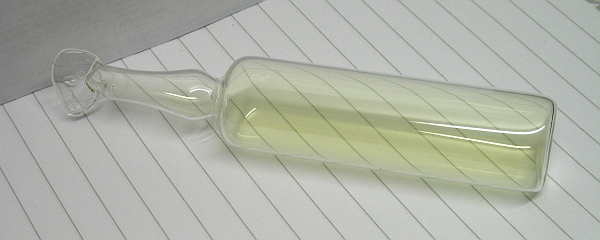
\includegraphics[height=2.9cm]{images/book2/chlorine.jpg}\hspace{0.5em}%
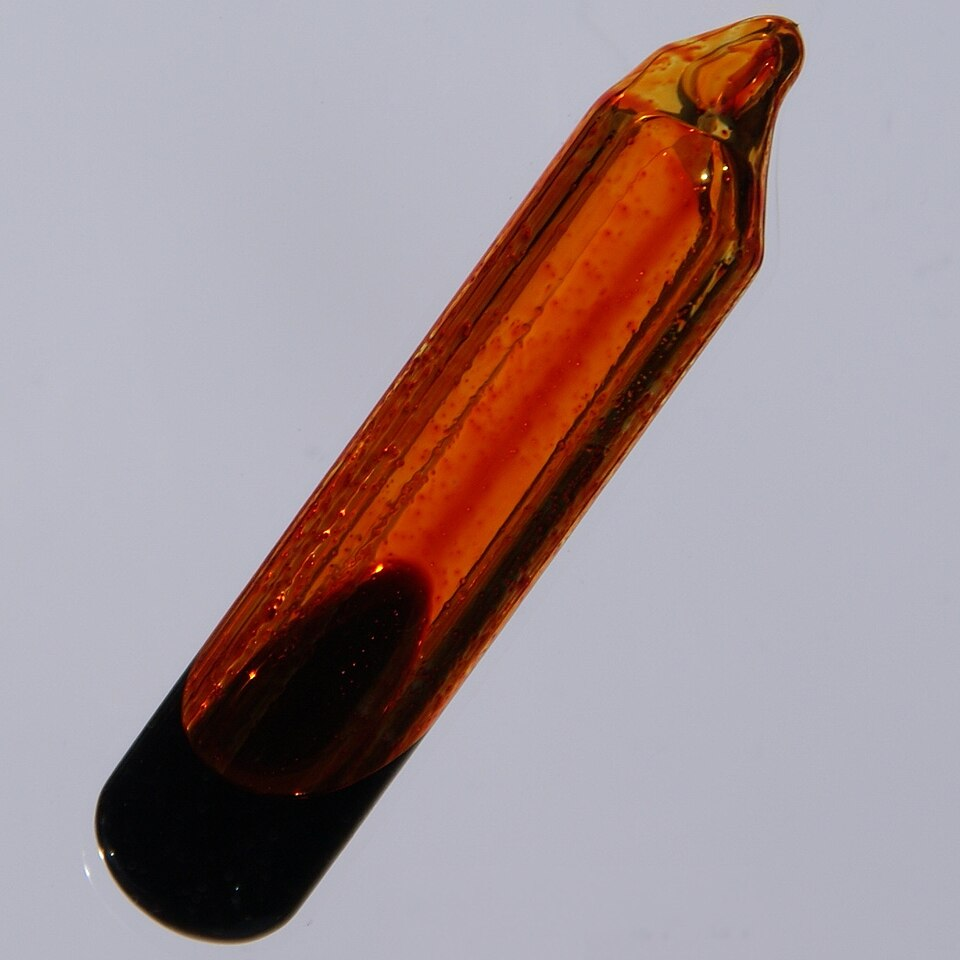
\includegraphics[height=2.9cm]{images/book2/bromine.jpg}\hspace{0.5em}%
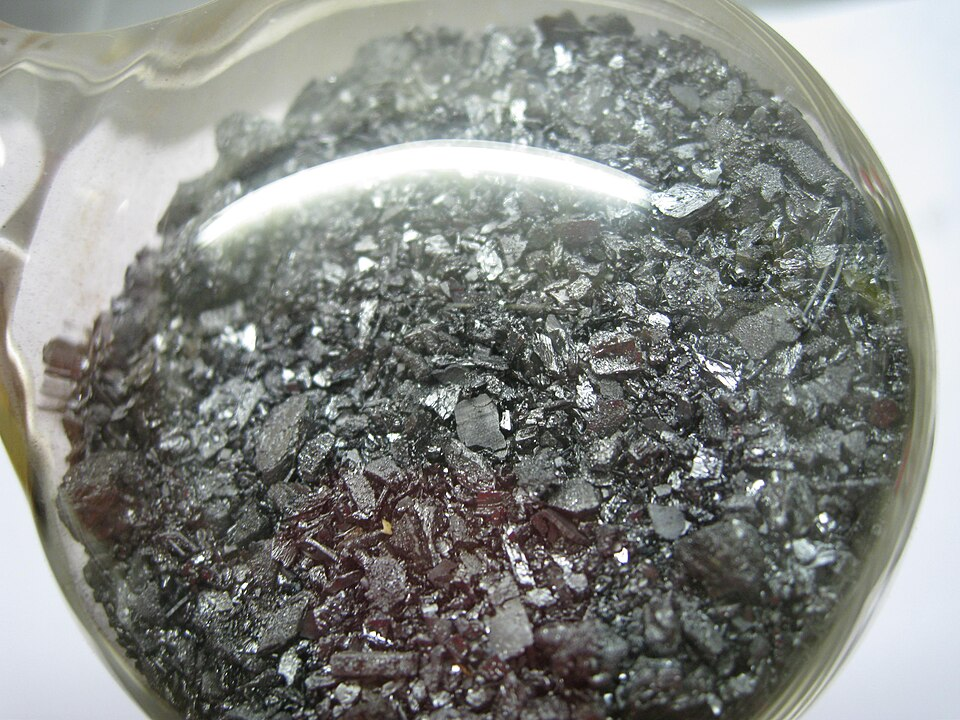
\includegraphics[height=2.9cm]{images/book2/iodine.jpg}

{\small क्लोरीन, एक हल्की पीली-हरी गैस (डब्ल्यू॰ ओएलेन, CC BY-SA 3.0);
ब्रोमीन, नारंगी वाष्प वाला एक गहरा लाल द्रव (यूरी, CC BY 3.0); आयोडीन,
धात्विक चमक वाले धूसर-काले \omterm{def:b1:crystals-metals:crystal}{क्रिस्टल} (डीएनएन87, CC BY 3.0)। क्लोरीन और
ब्रोमीन काँच की एम्प्यूलों में बंद हैं। सभी विकिमीडिया कॉमन्स।}
\end{omfigure}

\begin{proposition}[हैलोजनों की ऑक्सीकारक क्षमता]\label{prop:b1:p-block-16-18:halogen-oxidising-order}
\omterm{def:b1:p-block-16-18:halogen}{हैलोजन} ऐसे \omterm{def:b1:nernst:couple}{ऑक्सीकारक} हैं जिनकी प्रबलता समूह में नीचे की ओर घटती है:
$E^\circ(\ce{F2}/\ce{F-}) = 2.89$~V, \ce{Cl2}/\ce{Cl-} 1.36~V,
\ce{Br2}/\ce{Br-} 1.08~V, \ce{I2}/\ce{I-} 0.53~V। हर \omterm{def:b1:p-block-16-18:halogen}{हैलोजन} समूह में अपने नीचे के
हैलाइड आयनों को ऑक्सीकृत करता है।
\end{proposition}

\begin{proof}
मान हैलाइड आयनों की निर्माण गिब्ज़ ऊर्जाओं से आते हैं
(\cref{ch:b1:nernst})। गामा नियम के अनुसार, \ce{X2}, \ce{Y-} को तब ऑक्सीकृत करता है जब
युग्म \ce{X2}/\ce{X-}, \ce{Y2}/\ce{Y-} से ऊपर हो: उदाहरण के लिए
\ce{Cl2 + 2Br- -> 2Cl- + Br2}, $\log K = 2(1.36 - 1.08)/0.059 = 9.5$।
समूह में नीचे जाने पर परमाणु बड़े होते जाते हैं, अतिरिक्त इलेक्ट्रॉन के लिए उनकी बंधुता और
छोटे हैलाइड आयनों की जलयोजन-ऊर्जा घटती जाती है, और साथ में विभव भी।
\end{proof}
% ledger: dfg:F-_ao, dfg:Cl-_ao, dfg:Br-_ao, dfg:I-_ao

\begin{omfigure}
\begin{tikzpicture}
\begin{axis}[
  ybar, width=0.62\linewidth, height=5.0cm, ymin=0, ymax=3.3,
  symbolic x coords={F,Cl,Br,I}, xtick=data,
  xticklabels={\ce{F2}/\ce{F-}, \ce{Cl2}/\ce{Cl-}, \ce{Br2}/\ce{Br-}, \ce{I2}/\ce{I-}},
  ylabel={$E^\circ$ (V)}, bar width=16pt, nodes near coords,
  every node near coord/.append style={font=\scriptsize},
  tick label style={font=\small}, label style={font=\small}, enlarge x limits=0.2]
\addplot[fill=omThm!40, draw=omThm] coordinates {(F,2.89) (Cl,1.36) (Br,1.08) (I,0.53)};
\end{axis}
\end{tikzpicture}

{\small \qty{25}{\celsius} पर हैलोजन--हैलाइड युग्मों के \omterm{def:b1:nernst:electrode-potential}{मानक विभव},
सारणीबद्ध गिब्ज़ ऊर्जाओं से परिकलित: \omterm{def:b1:nernst:couple}{ऑक्सीकारक}
क्षमता समूह में नीचे की ओर लगातार घटती है।}
\end{omfigure}

हाइड्रोजन हैलाइड सभी जल में अम्ल हैं, पर \ce{HF} दुर्बल है
($\mathrm{p}K_a$ 3.16) जबकि \ce{HCl}, \ce{HBr} और \ce{HI} प्रबल हैं:
\ce{H-F} आबंध अत्यंत प्रबल है और छोटा फ़्लुओराइड आयन प्रबल
\omterm{def:b1:intermolecular-forces-solvents:hbond}{हाइड्रोजन आबंधों} में बँधा रहता है। फ़्लुओरीन सबसे अधिक विद्युत-ऋणात्मक तत्त्व और
सारणी का सबसे प्रबल \omterm{def:b1:nernst:couple}{ऑक्सीकारक} है; वह केवल विद्युत-अपघटन से प्राप्त होता है।
क्लोरीन के \omterm{def:b1:p-block-13-15:oxoacid}{ऑक्सोअम्ल} --- हाइपोक्लोरस \ce{HClO}, क्लोरिक \ce{HClO3},
परक्लोरिक \ce{HClO4} --- हाइड्रोजन-रहित ऑक्सीजनों की संख्या के साथ
अधिक प्रबल होते जाते हैं, जैसा सभी \omterm{def:b1:p-block-13-15:oxoacid}{ऑक्सोअम्लों} के लिए है (\cref{def:b1:p-block-13-15:oxoacid}); क्लोराइड और क्लोरीन के साथ
उनकी पारस्परिक क्रिया का मानचित्र \cref{ch:b1:e-ph-diagrams} में बनाया गया था।
% ledger: dfg:HF_ao, dfg:F-_ao

\begin{omfigure}
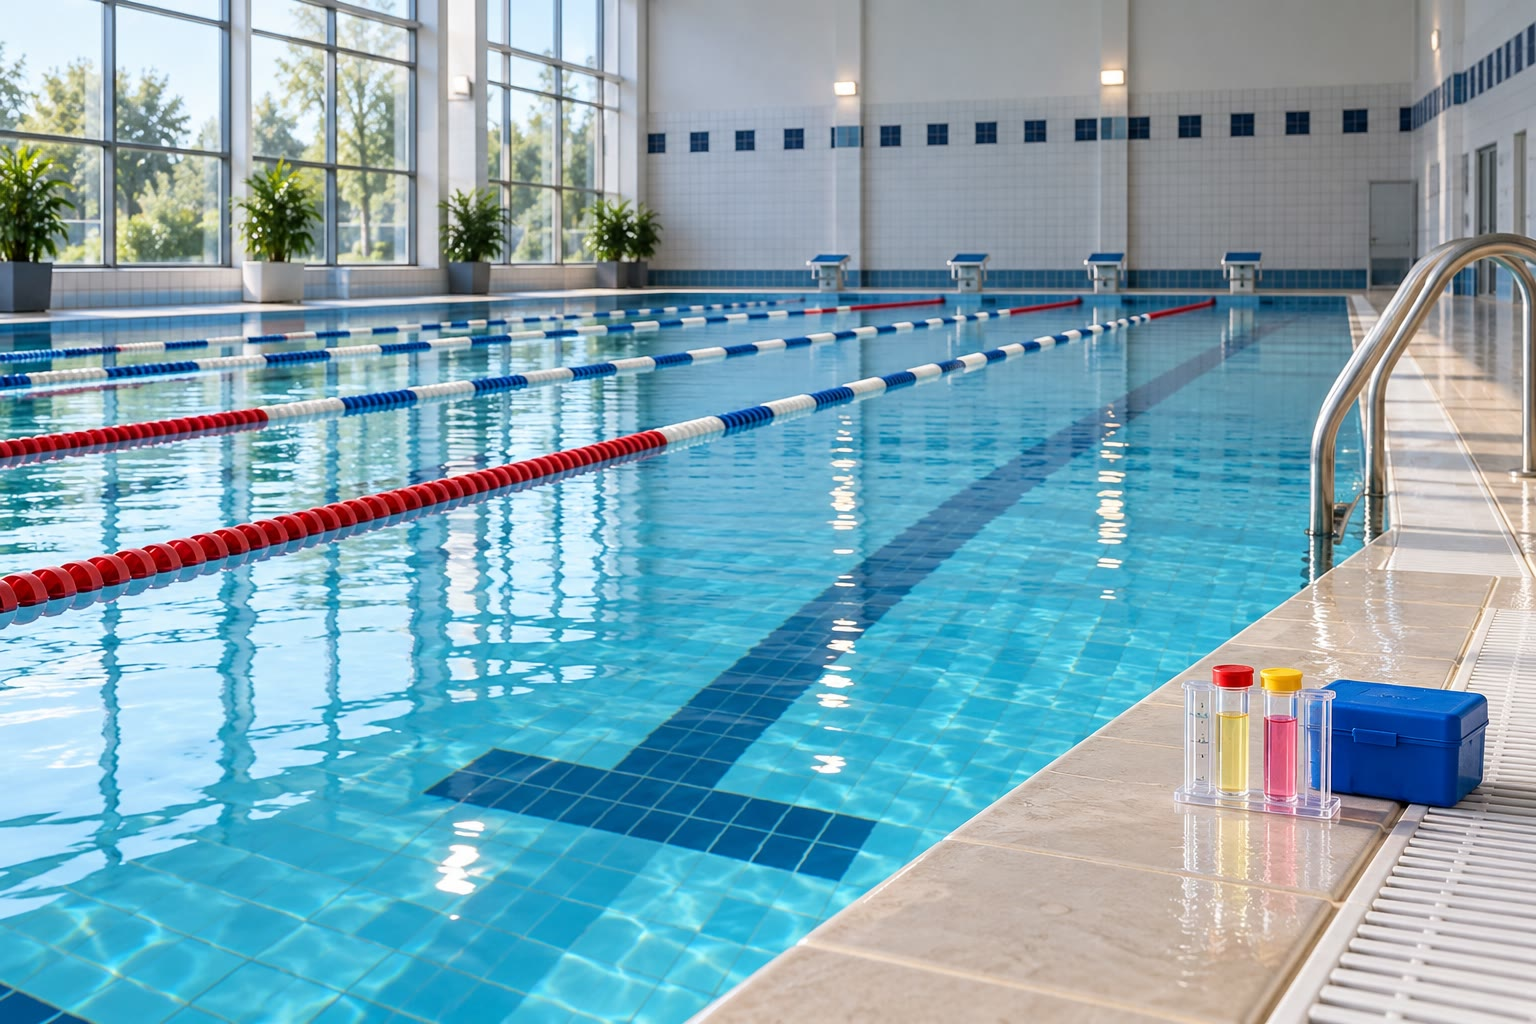
\includegraphics[width=0.55\linewidth]{images/book2/ai/b1-28-swimming-pool.jpg}

{\small एक सार्वजनिक तरणताल और उसकी जल-परीक्षण किट: हाइपोक्लोरस अम्ल के रूप में घुली
क्लोरीन की जाँच दिन में कई बार की जाती है।}
\end{omfigure}

\begin{definition}[अंतराहैलोजन यौगिक]\label{def:b1:p-block-16-18:interhalogen}
\emph{अंतराहैलोजन यौगिक}\index{अंतराहैलोजन यौगिक} दो भिन्न \omterm{def:b1:p-block-16-18:halogen}{हैलोजनों} का
यौगिक है: \ce{ICl}, \ce{BrF3}, \ce{ClF3}, \ce{IF7}। बड़ा,
कम विद्युत-ऋणात्मक \omterm{def:b1:p-block-16-18:halogen}{हैलोजन} \omterm{def:b1:complexation:complex}{केंद्रीय परमाणु} होता है, \ce{ClF3} और उससे ऊपर
विस्तारित अष्टक के साथ।
\end{definition}

\begin{inthelab}[हैलोजनों को संभालना]
क्लोरीन विषैली है और धूम-कोष्ठ में केवल थोड़ी मात्रा में
बनाई जाती है; ब्रोमीन त्वचा को जला देती है और उसकी वाष्प फेफड़ों पर आक्रमण करती है, और
उसका उपयोग तनु रूप में, धूम-कोष्ठ में, दस्तानों और चश्मे के साथ किया जाता है, और गिरे हुए अंश को नष्ट करने के लिए
सोडियम थायोसल्फ़ेट विलयन पास में रखा जाता है
(\ce{4Br2 + S2O3^2- + 5H2O -> 8Br- + 2SO4^2- + 10H+})। आयोडीन तीनों में सबसे
मृदु है, पर दाग़ लगाती है और ऊर्ध्वपातित होती है; उसे बंद बोतल में रखा जाता है।
\end{inthelab}

\section{उत्कृष्ट गैसें और उनके यौगिक}

उत्कृष्ट गैसों (He, Ne, Ar, Kr, Xe, Rn) के संयोजकता कोश भरे होते हैं और उनकी
आयनन ऊर्जाएँ अपने \omterm{def:b1:periodicity:table}{आवर्तों} में उच्चतम होती हैं (\cref{ch:b1:periodicity})।
लंबे समय तक अक्रिय मानी गई, भारी गैसें, जिनके बाहरी इलेक्ट्रॉन कम
दृढ़ता से बँधे होते हैं, सबसे अधिक विद्युत-ऋणात्मक तत्त्वों से अभिक्रिया करती हैं: ज़ेनॉन
\ce{XeF2}, \ce{XeF4}, \ce{XeF6} और ऑक्साइड देती है। उनकी आकृतियाँ ज़ेनॉन पर
\omterm{def:b1:lewis-resonance-vsepr:lewis}{एकाकी युग्मों} के साथ VSEPR नियमों का पालन करती हैं।

\begin{example}[ज़ेनॉन क्यों, आर्गन क्यों नहीं]
उत्कृष्ट गैसों की \omterm{def:b1:periodicity:ionisation-energy}{प्रथम आयनन ऊर्जाएँ} समूह में नीचे घटती हैं: He
24.59, Ne 21.56, Ar 15.76, Kr 14.00, Xe 12.13, Rn 10.75~eV। डाइऑक्सीजन की,
\ce{O2 -> O2+ + e-}, 12.07~eV है, लगभग ज़ेनॉन के बराबर। जो
\omterm{def:b1:nernst:couple}{ऑक्सीकारक} \ce{O2} से एक इलेक्ट्रॉन लेकर डाइऑक्सीजेनिल धनायन \ce{O2+} दे सके,
उसे इसलिए ज़ेनॉन को भी ऑक्सीकृत करना चाहिए, पर
आर्गन को नहीं, जो अपना इलेक्ट्रॉन 3.7~eV अधिक दृढ़ता से थामता है। ज़ेनॉन सचमुच
अत्यंत प्रबल \omterm{def:b1:nernst:couple}{ऑक्सीकारक} प्लैटिनम हेक्साफ़्लुओराइड \ce{PtF6} से अभिक्रिया करती है, और
समग्र संघटन \ce{XePtF6} वाला एक ठोस देती है, और स्वयं फ़्लुओरीन से भी, जो
नीचे की सारणी के ज़ेनॉन फ़्लुओराइड देता है। रेडॉन, जिसका आयनन और भी आसान है,
इतना रेडियोऐक्टिव है कि उस पर अधिक रसायन नहीं किया जा सकता।
\end{example}
% ledger: ie:He, ie:Ne, ie:Ar, ie:Kr, ie:Xe, ie:Rn, ie:O2, lit:XePtF6

\begin{omfigure}
\begin{tabular}{llll}
\hline
अणु & \omterm{def:b1:complexation:complex}{केंद्रीय परमाणु} पर इलेक्ट्रॉन युग्म & आकृति & मापा गया कोण \\
\hline
\ce{SO2} & 2 आबंधी क्षेत्र + 1 \omterm{def:b1:lewis-resonance-vsepr:lewis}{एकाकी युग्म} & कोणीय & \ang{119.5} \\
\ce{SF6} & 6 आबंधी & अष्टफलकीय & \ang{90} \\
\ce{ClF3} & 3 आबंधी + 2 \omterm{def:b1:lewis-resonance-vsepr:lewis}{एकाकी युग्म} & T-आकार & \ang{87.5} \\
\ce{XeF2} & 2 आबंधी + 3 \omterm{def:b1:lewis-resonance-vsepr:lewis}{एकाकी युग्म} & रैखिक & \ang{180} \\
\ce{XeF4} & 4 आबंधी + 2 \omterm{def:b1:lewis-resonance-vsepr:lewis}{एकाकी युग्म} & वर्ग समतलीय & \ang{90} \\
\hline
\end{tabular}

\smallskip
{\small विस्तारित अष्टक या \omterm{def:b1:lewis-resonance-vsepr:lewis}{एकाकी युग्मों} वाले कुछ \omterm{def:b1:periodicity:table}{p-ब्लॉक} अणुओं की आकृतियाँ
(जहाँ उपलब्ध हों, मापे गए कोण)। \ce{XeF2} के \omterm{def:b1:lewis-resonance-vsepr:lewis}{एकाकी युग्म}
त्रिकोणीय द्विपिरामिड की तीनों विषुवतीय स्थितियाँ घेरते हैं, जिससे अणु
रैखिक रहता है।}
% ledger: geo:SO2.aOSO, geo:SF6.aFSF, geo:ClF3.aFClF, geo:XeF2.aFXeF
\end{omfigure}

आर्गन, जो वायु का लगभग एक प्रतिशत है, प्रयोगशालाओं में और वेल्डन में क्रियाशील पदार्थों की
रक्षा करती है; हीलियम, जो प्राकृतिक गैस से मिलती है, अतिचालक चुंबकों को ठंडा करती है, जैसे
NMR स्पेक्ट्रममापियों के चुंबक (\cref{ch:b1:structure-spectroscopy})।
% ledger: air:Ar

\section{अभ्यास}

\begin{exercise}[$\star$]\label{exo:b1:p-block-16-18:1}
\ce{H2S}, \ce{S8}, \ce{SO2},
\ce{SO3^2-}, \ce{SO4^2-}, \ce{S2O3^2-} (औसत) और \ce{H2S2O7} में सल्फ़र की \omterm{def:b1:nernst:oxidation-number}{ऑक्सीकरण संख्या} बताइए।
\end{exercise}

\begin{exercise}[$\star$]\label{exo:b1:p-block-16-18:2}
इनमें से कौन-सी अभिक्रियाएँ होती हैं: पोटैशियम आयोडाइड के साथ क्लोरीन; सोडियम ब्रोमाइड के साथ
आयोडीन; सोडियम क्लोराइड के साथ ब्रोमीन; सोडियम ब्रोमाइड के साथ क्लोरीन?
जो होती हैं उन्हें लिखिए।
\end{exercise}

\begin{exercise}[$\star$]\label{exo:b1:p-block-16-18:3}
\ce{SO2}, \ce{SO3} और \ce{O3} की \omterm{def:b1:lewis-resonance-vsepr:lewis}{लुइस संरचनाएँ}, उनकी
\omterm{def:b1:lewis-resonance-vsepr:resonance}{अनुनादी संरचनाओं} के साथ, खींचिए और उनकी आकृतियाँ बताइए।
\end{exercise}

\begin{exercise}[$\star$]\label{exo:b1:p-block-16-18:4}
जल के साथ और सोडियम हाइड्रॉक्साइड के साथ \ce{SO2} और \ce{SO3} की
अभिक्रियाएँ लिखिए।
\end{exercise}

\begin{exercise}[$\star\star$]\label{exo:b1:p-block-16-18:5}
\qty{0.10}{mol/L} पर हाइड्रोफ़्लुओरिक अम्ल का pH परिकलित कीजिए और उसी सांद्रता पर
हाइड्रोक्लोरिक अम्ल से तुलना कीजिए। अंतर समझाइए।
\end{exercise}

\begin{exercise}[$\star\star$]\label{exo:b1:p-block-16-18:6}
VSEPR से \ce{BrF5}, \ce{IF7} (सात \omterm{def:b1:lewis-resonance-vsepr:lewis}{आबंधी युग्म},
पंचकोणीय द्विपिरामिड), \ce{ICl4-} और \ce{XeO3} की आकृतियों का पूर्वानुमान कीजिए।
\end{exercise}

\begin{exercise}[$\star\star$]\label{exo:b1:p-block-16-18:7}
\ce{Cl2 + 2I- -> 2Cl- + I2} का स्थिरांक परिकलित कीजिए और बताइए कि क्लोरीन
जल स्टार्च--आयोडाइड पत्र को नीला क्यों कर देता है।
\end{exercise}

\begin{exercise}[$\star\star$]\label{exo:b1:p-block-16-18:8}
दिखाइए कि ओज़ोन आयोडाइड आयनों को आयोडीन में ऑक्सीकृत कर सकती है, और अम्ल में
अभिक्रिया लिखिए। ओज़ोन को मापने में इसका उपयोग क्यों होता है?
\end{exercise}

\begin{exercise}[$\star\star$]\label{exo:b1:p-block-16-18:9}
सांद्र सल्फ़्यूरिक अम्ल सुक्रोस, \ce{C12H22O11}, को झुलसाकर काला कर देता है।
कार्बन तक \omterm{def:b1:alcohol-activation:dehydration}{निर्जलीकरण} लिखिए और \qty{10.0}{g} शर्करा से कार्बन का द्रव्यमान
परिकलित कीजिए।
\end{exercise}

\begin{exercise}[$\star\star\star$]\label{exo:b1:p-block-16-18:10}
दूसरी अम्लता को ध्यान में रखते हुए ($\mathrm{p}K_a = 1.99$) \qty{0.10}{mol/L} पर
सल्फ़्यूरिक अम्ल का pH परिकलित कीजिए। दूसरी अम्लता
कितना जोड़ती है?
\end{exercise}

\begin{exercise}[$\star\star\star$]\label{exo:b1:p-block-16-18:11}
विभवों का उपयोग करके समझाइए कि फ़्लुओरीन को जल में किसी भी रासायनिक \omterm{def:b1:nernst:couple}{ऑक्सीकारक} से
फ़्लुओराइड को ऑक्सीकृत करके क्यों नहीं बनाया जा सकता, और उसे जलीय विलयन के बजाय
किसी गलित फ़्लुओराइड के विद्युत-अपघटन से क्यों बनाना पड़ता है।
\end{exercise}

\begin{exercise}[$\star\star\star$]\label{exo:b1:p-block-16-18:12}
आयोडीन जल में केवल अल्प विलेय है पर पोटैशियम आयोडाइड
विलयन में ट्राइआयोडाइड आयन \ce{I3-} के रूप में घुल जाता है।
\ce{I2(aq)} ($\Delta_f G^\circ = \qty{16.40}{kJ/mol}$), \ce{I-} ($-51.57$)
और \ce{I3-} ($-51.4$) की गिब्ज़ ऊर्जाओं का उपयोग करके \ce{I2 + I- <=> I3-} का स्थिरांक परिकलित कीजिए।
\end{exercise}

\section{समस्या: एक टन सल्फ़र}

\begin{problem}[{सप्ताहांत समस्या --- सल्फ़र का दहन, सल्फ़र डाइऑक्साइड का उत्प्रेरकी
ऑक्सीकरण, अवशोषण और ओलियम, सल्फ़्यूरिक अम्ल की दूसरी
अम्लता, और एक टन सल्फ़र से बने अम्ल का द्रव्यमान}]
\label{pb:b1:p-block-16-18:1}
एक सल्फ़्यूरिक अम्ल संयंत्र प्राकृतिक गैस से पुनःप्राप्त सल्फ़र जलाता है। मोलर द्रव्यमान
(\unit{g/mol}): S 32.1, \ce{O2} 32.0, \ce{SO2} 64.1, \ce{SO3} 80.1,
\ce{H2SO4} 98.1, \ce{H2O} 18.0; वायु में आयतन से \qty{21}{\percent}
\ce{O2} है; $\mathrm{p}K_a(\ce{HSO4-}) = 1.99$; $R =
\qty{8.314}{J/(K.mol)}$।

\medskip
\noindent\textbf{भाग I --- सल्फ़र का दहन।}
\begin{enumerate}
  \item S, \ce{SO2}, \ce{SO3} और
        \ce{H2SO4} में S की \omterm{def:b1:nernst:oxidation-number}{ऑक्सीकरण संख्या} बताइए।
  \item सल्फ़र का दहन लिखिए।
  \item \ce{SO2} की \omterm{def:b1:lewis-resonance-vsepr:lewis}{लुइस संरचना} खींचिए और उसकी आकृति का पूर्वानुमान कीजिए।
  \item एक टन में सल्फ़र की मात्रा परिकलित कीजिए।
  \item केवल दहन के लिए वायु का आयतन (\qty{25}{\celsius}, \qty{1}{bar})
        परिकलित कीजिए।
  \item दाहक से निकली गैस को परिवर्तक से पहले ठंडा क्यों किया जाता है?
\end{enumerate}

\medskip
\noindent\textbf{भाग II --- उत्प्रेरकी ऑक्सीकरण।}
\begin{enumerate}[resume]
  \item \ce{SO2} का \ce{SO3} तक ऑक्सीकरण लिखिए।
  \item \qty{25}{\celsius} पर उसका स्थिरांक लगभग $10^{24.8}$ है। फिर भी
        \omterm{def:b1:elementary-steps:catalyst}{उत्प्रेरक} क्यों आवश्यक है?
  \item \cref{ch:b1:elementary-steps} की भाषा में वैनेडियम(V) ऑक्साइड की क्या भूमिका
        है?
  \item \ce{SO3} की आकृति खींचिए।
  \item आधिक्य वायु क्यों प्रयुक्त होती है?
  \item यदि रूपांतरण \qty{99.7}{\percent} हो, तो \ce{SO2} का कितना अंश
        नष्ट होता है?
\end{enumerate}

\medskip
\noindent\textbf{भाग III --- अवशोषण।}
\begin{enumerate}[resume]
  \item सल्फ़्यूरिक अम्ल में \ce{SO3} का अवशोषण लिखिए।
  \item \ce{SO3} सीधे जल में अवशोषित क्यों नहीं किया जाता?
  \item ओलियम का तनुकरण लिखिए।
  \item प्रक्रम का समग्र समीकरण लिखिए।
  \item प्रति टन सल्फ़र खपे जल का द्रव्यमान परिकलित कीजिए।
  \item अम्ल को जल में ही क्यों डालना चाहिए और कभी उलटा क्यों नहीं?
\end{enumerate}

\medskip
\noindent\textbf{भाग IV --- अम्ल।}
\begin{enumerate}[resume]
  \item दूसरी अम्लता को ध्यान में रखते हुए \qty{0.050}{mol/L} सल्फ़्यूरिक अम्ल विलयन का
        pH परिकलित कीजिए।
  \item \qty{99.5}{\percent} समग्र \omterm{def:b1:extent-q-and-k:fractional-extent}{लब्धि} के लिए सल्फ़्यूरिक अम्ल का
        द्रव्यमान परिकलित कीजिए।
  \item संसार ने 2025 में लगभग \qty{84}{Mt} सल्फ़र उत्पादित किया। यदि सब
        रूपांतरित हो जाए, तो वह सल्फ़्यूरिक अम्ल का कितना द्रव्यमान देगा?
  \item एक टन सल्फ़र (पूर्ण रूपांतरण) से प्राप्त हो सकने वाले सल्फ़्यूरिक अम्ल का द्रव्यमान
        बताइए।
\end{enumerate}
\end{problem}
